\myChapter{Corporate Security Solutions for BYOD}\label{chap:byodSotA} 

\begin{flushright}{\slshape
   ... } \\ \medskip
    --- {}
\end{flushright}

\minitoc\mtcskip
\vfill

\lettrine{T}{he} way how users employ their devices has changed in the past few years; even the number of different devices per user is increasing because of the so-called Internet of Things \cite{weber2010internet}. Thanks to it, users have more flexibility since they can now use their devices to access company assets and continue working outside of the workplace. To allow this way of working, companies have started to adopt what has been called the Bring Your Own Device (BYOD) philosophy.

But data security and privacy are key factors for a company, and thus, in order to protect them, it is usual that the Chief Security Officer (CSO) of a company defines a set of Organizational Security Policies \cite{Opp_Security11}. Allowing a BYOD environment implies taking care of the risks that the use of personal devices can bring to
the company \cite{gangula2013survey}. For instance, the mixture between personal and professional information in these devices would allow the user to navigate inside social networks, where important data could be leaked in the event of a security incident.  

In this scenario several solutions that manage corporate security have appeared. Most of them are geared for both smartphones and desktop PCs, although some are implemented only for a certain platform. However, almost all of them try to be non-intrusive with regards to users' personal data, friendly, and easy to use.

Even with the help of those solutions, it has been demonstrated that employees who ignore company security policies are the main hazard for company security \cite{Adams_Users05}. In this situation, the tools that are appearing in the market aim to cope with the concept of seamless working experience on different devices. This concept is a methodology of work which allows users to start, or continue a working session, over multiple devices and locations, without any significant loss of data. This new situation has a big impact from the point of view of the security \cite{Schu_SecPatterns05}, since company data borders have changed in the last years. Therefore, now the users can access important data from outside the enterprise, and possibly through a non completely secure channel.

As mentioned earlier, in the introduction, the aim of this thesis is to create a methodology that extracts knowledge and present it in the form of rules that the CSO can include in the initial, fixed set of security policies. To this end, in this chapter we start by giving numbers about the usage of personal devices by the workforce during working time, and how are the companies coping with the BYOD philosophy. Also, in this chapter we we propose a taxonomy to classify the features of BYOD systems. This taxonomy is used to present an overview of BYOD security solutions. Finally, we introduce a BYOD system named MUSES, from Multi-platform Usable Endpoint Security, which is being developed within an European Project\footnote{\url{http://musesproject.eu/}} of the same name. MUSES is a dev\-ice\--in\-de\-pen\-dent end-to-end user-centric tool, based on a set of security rules defined as specifications of the Corporate Security Policies. Then, a comparison between these tools and MUSES is conducted, focusing on the advances beyond the state of the art that this novel system includes.

\section{Preliminary concepts and background about enterprise security}
\label{sec:preliminaryconcepts}

One of the tasks of a CSO is to elaborate an efficient set of Information Security Policies (ISPs), for controlling a certain, and already known, structure \cite{Opp_Security11}. This means that, until the appearance of BYOD, enterprises used to follow static security policies devoted to control an environment where the company assets and the devices were purchased and maintained by the company. Now that corporate networks are becoming dynamic for being adapted to this BYOD philosophy, there is an additional risk as employees' devices are not always company-owned. This means that the CSOs have to find the balance between having a fast response to any user action that might cause harm (in terms of money loss because of a security incident), and trying not to intrude into users' privacy. A needed security policy, or in this case, an ISP should deal with the way of protecting a certain organization's information against a security breach. Though there are standards, such as the ISO27002 or the Security Forum's Standard of Good Practice\footnote{\url{https://www.securityforum.org}}, and many guidelines \cite{SecPol09}, an ISP should be adapted depending on the characteristics of the community or organization that they are built for. In this sense, MUSES stands up for a self-adaptation of company security policies.

On the other hand, employee-owned devices like smartphones, can be both used for personal matters at work, and for continuing working outside of the workplace. Smartphones are more than simple mobile phones, and people who use them in their works have the possibility of maintaining a good balance between work and private life. For this reason, the risk of uncontrolled devices accessing to corporate assets in unsafe conditions, due to the number of new risks which are linked to smartphones \cite{gangula2013survey}, is increasing.

Usually, the enterprise network architecture is being adapted to cope with external attackers \cite{MIT05}. However, with the incorporation of BYOD, the threat is about corporate assets being compromised due to employees' devices with vulnerabilities \cite{android11}, or leaked because they are being accessed from a device connected through an insecure (public) network.

Thus now, more risky situations should be considered when designing a company's network architecture. Figure \ref{fig:proposed_diagram} shows the proposal that can be used to start the study of solutions that may secure such a dynamic environment. It includes the possibility of having employee-owned mobile (smartphones and tablets) and portable (laptops) devices, and also the opportunity that the employees have of connecting these devices either from inside or outside the company premises. Moreover, company's information assets are constantly accessed under these conditions, considering that an information asset means every \textit{piece of information} that has a \textit{value} (cost depending on the risk of being lost or leaked) for the company. It can be referred to files with sensitive information, as well as confidential mails, or even to company applications.

\begin{SCfigure}[tb]
\centering
	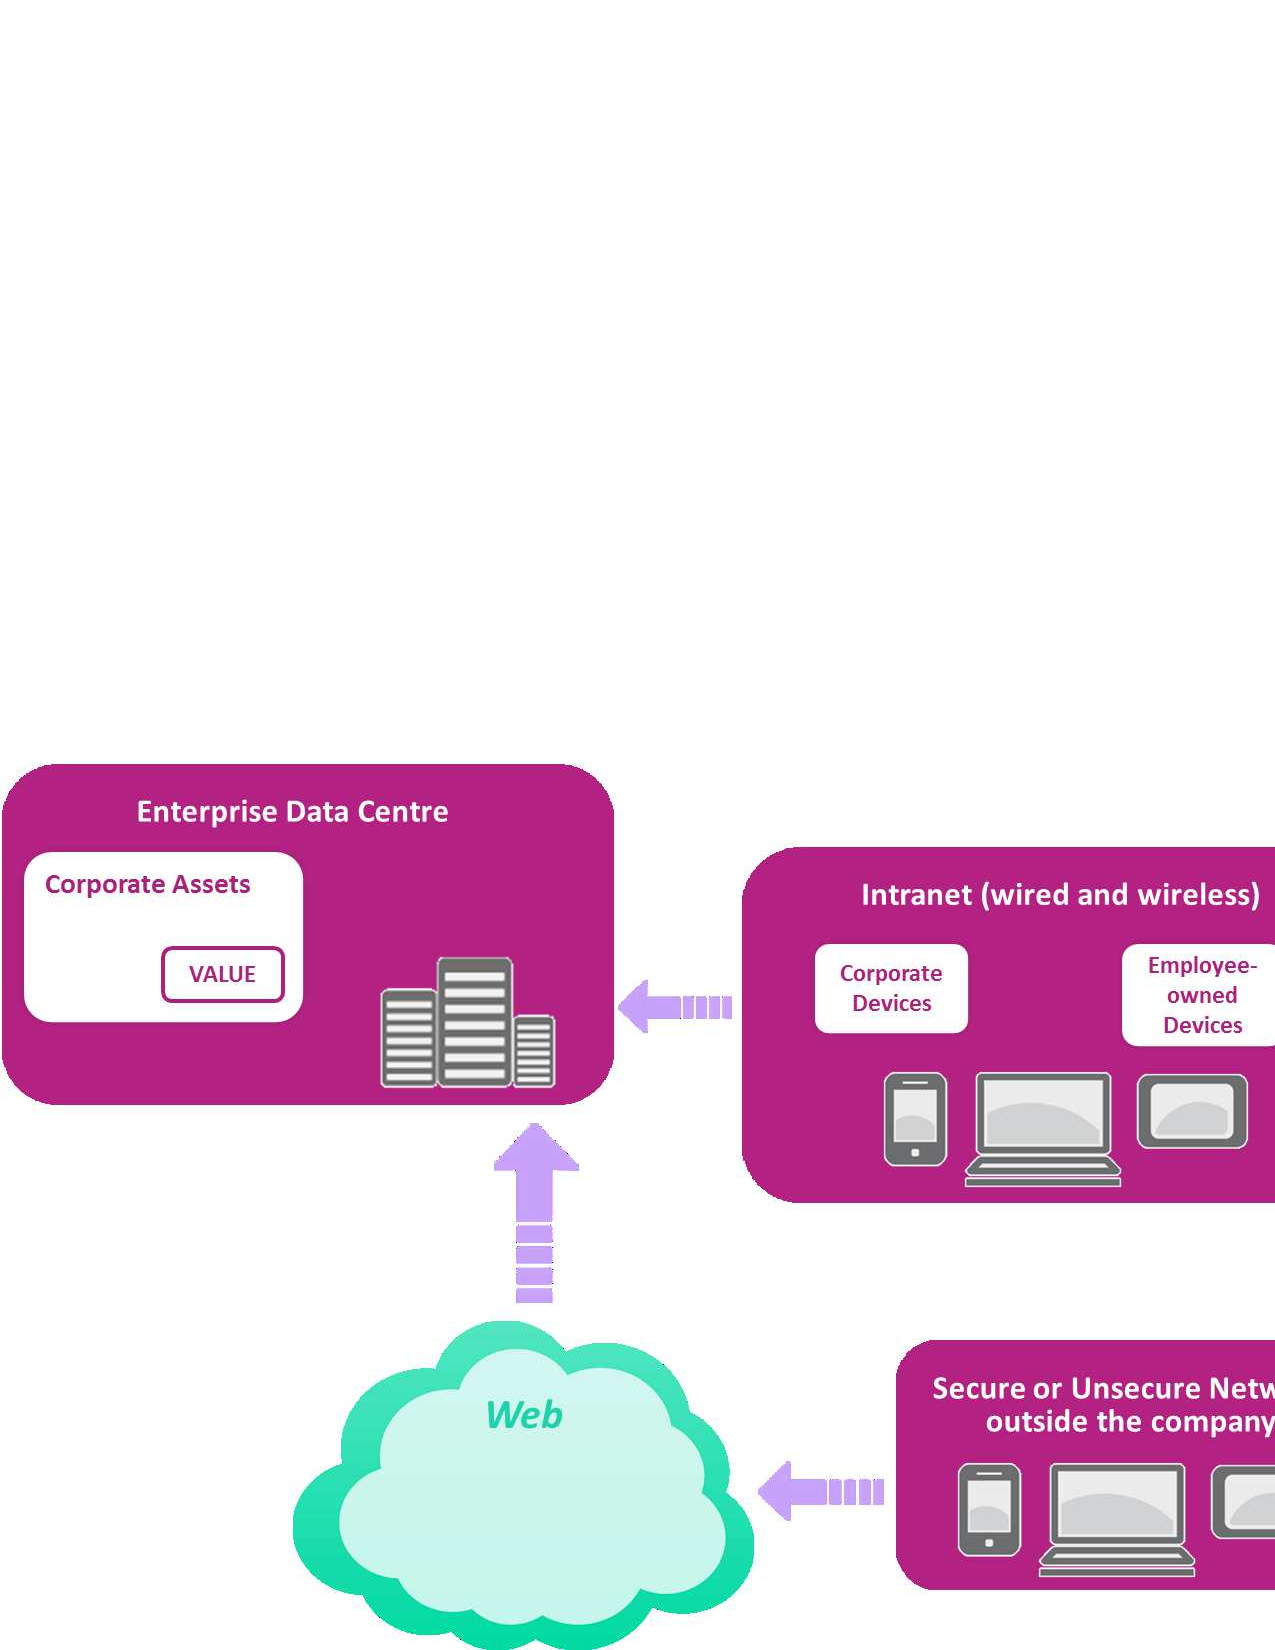
\includegraphics[scale =0.4] {gfx/byodSotA/proposedDiagram.pdf}
	\caption{Architecture approach of an enterprise network, assuming that it has adopted the BYOD philosophy.}
	\label{fig:proposed_diagram}
\end{SCfigure}

The other issue to cope with is the elaboration of a good ISP, understandable for every user of the company, and more importantly, non-intrusive for them. A lot of researchers have studied the natural tendency of employees to comply with the ISP \cite{SecPolComp10,SecPolComp12,SecPolComp14}, reaching conclusions such as the employees compliance with the security policies increases educating or training them in information security awareness \cite{SecPolComp09}, and decreases applying too much sanctions when a misuse or abuse occurs \cite{SecPolPenalty09}. Thus, in this chapter, for each reviewed tool we specify if the developers have taken into account the construction of ISPs, or if they give some guidelines for building them. 

This situation leads to a need of protecting the organization's side, but also the users' side, making non-interfering easy-to-follow ISPs, and leaving them to use their devices for personal purposes while working, without putting organization's information assets under risk. The compliance of these requirements would compose an End-to-End Security Solution (protecting both enterprise and employee), which is the motivation of the commented tools and, as will be detailed, is the aim of the MUSES project.

Besides, there is an emerging research area in the field of BYOD. This is because, as it has been mentioned, it is becoming a growing trend \cite{Garba15organisational}. There exist several methodological works on this subject. Samaras \cite{Samaras13SaaS} proposes a methodology design of a security architecture taking into account their logical design, logical architecture, security mechanisms and physical architecture. First, the business processes are studied and legal and security requirements are analyzed. After applying several controls the architecture is validated using different criteria: Correctness, Completeness, Usability and Flexibility. Romer \cite{Romer14BestPractices} proposes a set of best practices for BYOD security: centralize control and monitoring, protect confidential devices, increase trust with private clouds, connect to important services (such as Dropbox), block risky services and choose proven solutions.

Although some works present studies on the impact of BYOD in privacy \cite{Miller12Privacy} or relationship between workers productivity and stress \cite{Haejung12Door}, the most of them are focused in describing new systems and concepts in this paradigm. Scarfo presents in \cite{Scarfo12survey} a survey about the coming up methods in BYOD security. This survey summarizes the research in two different approaches: {\em hands-off} versus {\em hand-on} devices. The first one proposes the use of some kind of virtualization or wrapping of the applications, while the latter is based in a tight control and monitoring of the device by the company.

An example of hands-off method is presented in the work by Gessner et al. \cite{Gessner13userfriendly}. This work mentions the importance of avoiding the modification of the underlying operating system (OS). Therefore, they propose the use of a ``container'' application, installed in the mobile device. This container is able to execute inside it the enterprise applications, acting as a barrier with the rest of the applications, and allowing direct communication with the enterprise VPN. The combination of this method, along cryptographic protocols and time-based sessions, offers a trade-off between security and usability. Also, this method avoids the modification of the underlying kernel of the device.

Other works propose the analysis of the applications before being installed. For example, in \cite{Armando14metamarket} a meta-market application is used to supervise the installation of new applications, using static analysis and code instrumentation techniques, taking into account the organizational security policies. A meta-market prototype is tested with Google Play market using a real world BYOD security policy \footnote{The US Government BYOD security guidelines.}.

It is interesting to mention that previous works are mainly focused in separating into hands-off vs hand-on devices, or static analysis techniques. However, neither of the papers found in bibliography establishes a taxonomy. In addition, the tools described in the reviewed works, do not implement any security policies adaptation methods, as the system that we present in this paper.

\section{Tools for corporate mobile security}
\label{sec:toolsreview}

Many tools for companies, as well as for devices, have adopted the BYOD have been released in the past four years. This way, and more focused on the enterprise, there are some tools which offer the CSO ways to control the devices which enter into the system, for instance, and also to protect the employees' data by means of data encryption and data protection by requiring the use of strong and secure passwords. Other tools for managing a BYOD situation add to their features guidelines for the CSOs to develop good ISPs, like Good's BYOD solution (see Section \ref{subsec:othertools}). On the other hand, many solutions have been presented which are more focused on the device side, although they implement also the server side. This is the case, for instance, of Android for Work (see Section \ref{subsec:androidwork}). Some of those tools have influenced the development of the MUSES system  itself (Section \ref{sec:muses}), which can complement them, as adds other features that go beyond the state of the art. 

The products that have been reviewed were chosen either because they have appeared in top-10 web articles \footnote{\url{http://www.networkworld.com/article/2357899/data-center/108866-10-Mobile-Device-Management-Leaders-That-Help-IT-Control-BYOD.html#slide11}}, or they have been developed for the main smartphone platforms \footnote{\url{http://www.idc.com/prodserv/smartphone-os-market-share.jsp}}. Actually, the selection process have been difficult, as some of the initially found tools or companies in the web were bought by others that we do review here. Also, because this market is still growing, there are not many solutions to review, and here we display the ones more alike to MUSES. This section introduces the most relevant features of these products, as they can be considered related to the MUSES objectives.

As these tools have several access levels, different detection methods, or diverse data control, there exist a number of aspects that the end-users need to take into account to validate if a product fits their needs. Therefore, we propose the next taxonomy in order to classify the BYOD tools described in this paper.

\begin{itemize}
\item {\em Online or offline threat detection method}. This kind of tools can identify security threats during runtime (online) or before their implantation (offline). For example, using some kind of DM technique, such as classification methods, or merely the system administrator experience, can be used to generate rules before the deployment of the tool (offline) to detect threats in runtime. However, new rules cannot be added. On the contrary, a real-time adaptation using actual data sources, that modify the parameters of the detection system, follows an online scheme.
\item {\em Updatable or fixed information database}. This classification is related to the previous one. New information gathered by the system during runtime can be stored in a database to generate new rules. If this database is not changed during runtime, as in the offline example explained above, the database is {\em fixed}. An example could be the hand-coded rules of a firewall, such as {\em iptables}, obtained from an offline method. On the other hand, an updatable database, such as the system logs, that can be used to extract new information, may offer more valuable data source for dynamic adaptation mechanisms. However, it is not mandatory for an online threat detection method to use an updatable database, as current data may be analyzed and deleted once a new rule is created. 
\item {\em Based in an external service or standalone}: A standalone tool do not require a external service to be used. For example, a basic firewall. However, as mentioned by \cite{Romer14BestPractices} in previous section, a service for threat monitoring, or a private cloud usage are good practices to apply in BYOD.
\item {\em Invasive or non-invasive data access}. A system can be considered {\em invasive} if a user must use a certain tool to perform their job. For example, opening a specific browser provided by the tool, instead of the original device browser, such as Chrome of Safari. An example of an invasive marketplace is the one proposed by \cite{Armando14metamarket} and discussed in previous section. Instead, a {\em non-invasive} data access is transparent to the user. An example is a log analyzer daemon that updates other program configurations or sends information to the company server.
\item {\em Superuser or non-superuser system control}. Using a tool in superuser mode would add more information and control than a non-superuser running mode, as it can access to elements of the device usually forbidden for regular applications, such as network, logs or other devices. However using superuser control may lead to a lack of user privacy, as explained in \cite{Gessner13userfriendly}.
\end{itemize}


%----------------------------------------------------------------------------

\subsection{IBM Mobile Security}
\label{subsec:ibm}

One of the first companies who supported the BYOD model was IBM \cite{IBM_tool}, as they recognized the increase of employees who brought their personal smartphones or tablets into the workplace \cite{ibm11}. IBM provides different solutions divided into ``technology solutions'', and ``services'', and almost all are are mainly focused on the management of the devices in the system. Then, it might seem clear that the first disadvantage is not including all features in one system, but to make the companies choosing between one or another, or invest even more resources instead.

Main services offered by IBM can be divided into three categories: Mobile Enterprise Services, Hosted Mobile Device Security Management, and Enterprise Wireless Networks. However, here we only discuss the former, because it is the only one related to BYOD. Mobile Enterprise Services is offered as an integrated solution for smartphones and tablets as well, but then it is divided in different sub-services that the company has to acquire separately. Some of them are related, to cloud computing. Among them, there is one which is interesting for the scope of this paper, the so-called `hosted vulnerability management'. This sub-service seems to implement one of the most important advantages of the MUSES system, the self-adaptation. IBM performs deep scans over the security incidents data, either by computer forensics analysis, if the incident happened, or by normal data, if the device was enough secure. They claim in their website \footnote{\url{http://www-935.ibm.com/services/us/en/it-services/security-services/vulnerability-management/}} that their tool is able to recognize new vulnerabilities or threats with enough accuracy. 

%FERGU: HABLANDO DE LOS PRODUCTOS
The specific IBM products related to BYOD security are included in their {\em MobileFirst} \footnote{\url{http://www.ibm.com/mobilefirst}} suite. MobileFirst is a set of mobile applications and services, based in big data analytics and cloud computing. It includes several products, such as a framework for app development (MobileFirst Platform), a Platform as a Service (BlueMix) or a threat detection system (Trusteer Rapport). %FERGU: sí, es rApport, no rEpport, no lo cambiéis :P
 However, the most interesting one with respect to this work scope, is {\em MobileFirst Protect}. This product, formerly known as {\em MaaS360} \footnote{\url{http://www.maas360.com/}}, is an MDM (Mobile Device Management) software to secure, monitor, and manage mobile devices. It uses a web portal in order to centralize the security and control policies. This allows the deployment of applications or backups, among other possibilities. However, MobileFirst Protect seems a typical MDM tool, which just applies the existing set of security policies. No further risk and trust analysis is performed, neither is included a refinement of the rules derived from the policies.

The main difference with MUSES in this case, is that MUSES includes the threat recognition feature feature in the system, without the need of purchasing the service separately and configuring the different parts. Another difference is the fact that IBM software is not open source as MUSES system is. Then, to verify the success of this feature is highly difficult, as they do not present statistics in their website either. In addition, this product also offers the possibility to work offline, though an initial online authentication is needed \footnote{\url{https://developer.ibm.com/mobilefirstplatform/documentation/getting-started-6-3/authentication-security/offline-authentication/}}. 
 
%----------------------------------------------------------------------------

\subsection{Sophos Mobile Control}
\label{subsec:sophos}

Contrarily to IBM's solution services, Sophos offers a whole product for securing BYOD environments, which is called Mobile Control \cite{Sophos_tool}. It is oriented to IT administration for mobile devices, and it can be deployed in two ways: on-premises, which means that all data and services remain in the servers of the company, and as Software as a Service (SaaS), so that the services are provided through Lightweight Directory Access Control (LDAP). LDAP is an application protocol for accessing and maintaining distributed directory information services over an Internet Protocol (IP) network.

The tool manages all employees' smartphones and tablets from a single-based console. This console monitors the devices since the initial set up and registration, until they log off. Remainder features are similar to IBM's product, adding some new such as the incorporation of a service called Malware and Web protection, so that there is no need for having a previously installed antivirus in the devices. Also, version 4.0 adds a new version of what has been called `Sophos Antivirus Engine', with offline detection capabilities.

With regard to compliance enforcement, the main goal of this Mobile Control tool is to give more importance to company security, instead of giving more flexibility to the users. But it has been demonstrated by Herath and Rao in \cite{SecPolPenalty09} that this practise can result in bad users' behavior, even if it was not on purpose. Thus, the company BYOD initiative should include an acceptable use policy to ensure that the users are aware of the measures that the company would take if a device breaches any ISPs. Sophos aims to reach this by doing three main tasks: First, by allowing setting up user and group-based security policies separately. Secondly, by a risk mitigation in which the actions to perform can be set according to the severity of the breach. For minor cases, the company might want to simply inform to the user, but if sensitive data is at risk, a remote wipe might be the chosen option. Finally, compliance check, by constantly performing scans to detect malware and putting the devices in quarantine when they are found infected.

Thus, given the fact that this tool is more focused on the company
than in the user, it is worth to compare it to the MUSES system, as
the latter tries to focus on the users, being user-centric. This means
that is preferred to let the user know about a risky situation, rather
than making them feel ``watched''. 

%----------------------------------------------------------------------------

\subsection{Samsung KNOX and Blackberry Balance}
\label{subsec:samsungblackberry}

Even though these two tools are provided by two different manufacturers, Samsung and Blackberry, they both have in common their situation, as they found problems in the market in spite of their features. On the one hand, Blackberry sales have been decreasing since 2010 \cite{Blackberry_sales}.
On the other hand, Samsung revealed at the Barcelona Mobile World Congress 2013 the KNOX application \cite{Samsung_mwc13}, which was expected to be available for its last Galaxy smartphone generation. Then, it was delayed and again presented in the same congress in 2014 \cite{Samsung_mwc14}, but still remained delayed until it was apparently found insecure \cite{Samsung_insecure}. Finally, Samsung decided to collaborate with Google in Android Work \cite{Samsung_android}, as mentioned in Section \ref{subsec:androidwork}.

With regard to their features, Samsung KNOX, as well as Blackberry Balance, are more focused on the device side, while the solutions mentioned in previous subsections were more centered in being tools for CSOs. This also means that they are not device-independent, as KNOX is only for Samsung devices and Balance is integrated in BlackBerry 10 \cite{Blackberry_tool}. Looking at their situation and problems, it could be thought that making a BYOD solution platform-dependent is counteractive, which is why MUSES is independent of the device platform.

The main feature of KNOX is the use of different containers, or environments, for business and personal sides. Each one includes its own graphical configuration, such as wallpapers, or colour themes, in order to be more easily recognized and distinguished by the user.
A password is required in order to enter into the business side and, once \textit{logged in} to this container, no more passwords are needed for the business applications. The applications approved by the company IT department must meet Samsung security standards and, though it has been said that KNOX is a device-focused solution, the company offered an API. This API would allow the company to access to over almost 205 predefined IT policies. With regard to information protection methods, data files saved by applications of each environment are encrypted with AES 256-bit algorithm, in such manner that only the appropriate container can access these files. In the same way, the user is not allowed to share data between the two environments. 

Features in Blackberry Balance are similar. This security package was announced as a feature of BlackBerry 10. Nevertheless, it is available with BlackBerry Enterprise Service 10, which is a device management, security and app management for BlackBerry, iOS and Android devices. It is necessary to activate BlackBerry Balance for having available some security features, all related or similar to the aforementioned. For instance, a message is displayed when the user tries to copy work data and then paste it into personal apps. Also, a user attempting for actions that are not permitted in the company ISP, or may cause secure work information to be in contact with personal applications, these actions will not be permitted. 

On the other side, while KNOX allows to \textit{push} policies from the server to the devices, so they are available offline, Blackberry Balance only allows to read documents in this mode. Finally, another known feature is also offered by Blackberry, so if the device gets lost, it is stolen, or if the employee leaves the organization, there is an option to wipe just work information which can be done remotely.

As a summary, Blackberry Balance has little opportunity if Blackberry sales continue to decrease, as well as Samsung KNOX, which is still out of the market. With this situation, MUSES could be a good choice, because is device-independent, and is available as an open source tool for both devices and servers.

%----------------------------------------------------------------------------

\subsection{Blackphone}
\label{subsec:blackphone}

On the device side, one of the most powerful solutions found in the BYOD state of the art is, apparently, to directly use a phone which has been developed with data security in mind such as the BlackPhone \cite{Blackphone}. It has its own Android-based operating system, called \textit{PrivatOS} \cite{Blackphone}, which includes a privacy-focused application store, called \textit{Silent Store}, that takes care of the problem of applications which ask for certain permissions that can lead, for instance, to personal data leakage \cite{gangula2013survey}. BlackPhone also allows a remote wiping of the data if the device is lost or stolen. The main disadvantage of this solution is either the enterprise having to make an investment and buy these smartphones to the employees or to make employees buy them, so they cannot use the device they already have. Both options are against the BYOD philosophy. On the contrary, the MUSES system proposed in this work is designed as device-independent.
Furthermore, the lack of information about this system makes it difficult to determine its real qualities.

%----------------------------------------------------------------------------

\subsection{Android Work}
\label{subsec:androidwork}

This tool is the Google approach in the mobile enterprise security area, and  will run on Android 5.0 ``Lollipop''. It follows the idea of containers, previously presented in the Samsung KNOX description. Thus the container will be used to manage (encrypted) corporate data, and also to restrict what the users can do with them. This is called a ``dual-persona'' smartphone \cite{AndroidWork_review}.

This system is be strongly related to the Google Play market, as the applications will be `categorized'. Thus, Android Work provides the CSOs with a tool to define which apps would be allowed for being installed by the users and considered as corporate-related applications. Several enterprise-security aimed applications will be offered in the market, so the IT can decide which ones will be installed in the employees' devices. Also, they can manage the updates of these apps, in order to ensure that all the employees are up to date. For instance, one app could manage the creation of personal and work profiles, so the user just could access corporate assets after login in into the app. Moreover, the enterprise IT department could define specific security policies on these apps, in addition to the inherent protection that the container provides. However, the specifications of this tool \cite{AndroidWork_tool} do not include the ``self-adaptation'' as a feature, as the MUSES system does. 

Even though it does not analyze the system information for security rules evolution purposes, it offers policy management. Thus, the system will provide a framework for IT staff to manage business devices, but also, and more importantly, personal devices being used in a BYOD context. The CSO would give the employee an activation code in order to `connect' the smartphone to the enterprise and use this Android Work.
Therefore, IT admins will be able to specify which Google Play apps will be available for users to install through this work profile, including being able to provision apps to specific individuals or groups inside the company.

In addition to the work profiles, there will be considered other high-level ones with the ability to administrate the device from the corporate-security point of view, or as the owner, with all the privileges on the device.

Android Work presents only one advantage over MUSES, and roughly over all solutions, which is the ability to act over the Android kernel. The rest of tools only have permission for monitoring the running processes in the devices, while Android Work has, for instance, the ability to provide a `work' version of its native apps. MUSES, instead, depends on the developers to adapt their applications through a MUSES API, transforming them to MUSES Aware apps, as will be explained in Section \ref{subsec:client}. In any other case, and most of all with the ``self-adaptation'' feature of MUSES, it can be said that MUSES presents more advantages than the Google solution.

%----------------------------------------------------------------------------

\subsection{Other tools}
\label{subsec:othertools}

There exist other corporate security-aimed tools inside the BYOD philosophy, of which there are less references on the Internet, but still we consider important for having similar features as MUSES. These tools are:

\subsubsection{WSO2 - Enterprise Mobility Manager}

WSO2 Enterprise Mobility Manager (WSO2 EMM) \cite{WSO2_tool} is an open source platform that also works with the BYOD program. Some of this WSO2 EMM key features are:
% Antonio - cambio esto porque las negritas no se suelen usar apenas y para mantener la concordancia en formato con el resto de listas
\begin{itemize}
  \item \textit{Mobile Device Management}: It is used to manage both user and corporate owned devices, providing support for Android and iOS at the moment. It should be noted that this tool allows tracking every enrolled device, as well as obtaining reports and analytics of their use.
  \item \textit{Mobile Application Management}: With regard to the software, this platform is able to allow or deny the use of applications on enrolled devices based on the role of the user or policies, thus restricting the use of some apps to certain users.
  \item \textit{Enterprise App Store}: This store provides users with both enterprise and public applications approved by the company.
  \item \textit{Mobile Data Security}: WSO2 also allows the user's data to be encrypted via password.
\end{itemize}

Although this tool also includes features such as device location, remote wipe, or encrypt storage, its main disadvantage is that it does not work in offline mode. In the documentation \footnote{\url{https://docs.wso2.com/display/EMM200/Working+with+Policies}}, it is clearly stated that the policy compliance can be monitored while the devices are connected to the WSO2 EMM server. In addition, this tool seems to be only an MDM, without any refinement of the security policies.

\subsubsection{Good's Bring Your Own Device solution}

The philosophy followed by Good \cite{Good_tool} is similar to Samsung KNOX one: to create a secure container that places an unreachable partition between personal and business data in order to protect company assets. The solutions that they offer \cite{Good_tool} are similar than in the already described solutions. Their solution has been developed for the main OSs: iOS, Android, Windows phone, and also desktop computers with Windows. A Good's secure Network Operations Center (NOC) is introduced for dealing with the unauthorized devices, or for providing access to secure collaboration solutions (email, documents, calendar), the intranet, and both in-house or third-party mobile applications. Finally, Good offers best practice recommendations to help the company developing BYOD policies. A document can be accessed from Good's webpage \cite{Good_tool}, which contains several questions about ISPs and how to cope with all of them.

\subsubsection{Azzurri - Icon Mobilise}

It is a cloud-based service \cite{Azzurri_tool} to manage enterprise devices from the BYOD point of view, protecting sensitive corporate data and also letting the users enjoy them privately, by outsourcing the management of those devices to Azzurri.
 
\begin{itemize}
\item It offers a central deployment, administration and security control of all mobile devices regardless of their OS. %FERGU: securing como palabra no. security control mejor?
%Cambiado
\item It manages and enforces security policies `over the air' for both corporate and employee-owned mobile devices.
\item It does it by enforcing passwords and providing mechanisms for remote lock.
\item It offers the ability to wipe, even selectively, corporate data email and contacts on the device if lost or stolen.
\end{itemize}


\subsubsection{Citrix - XenMobile}

XenMobile with the development environment called Worx App SDK, made by Citrix Systems, provides BYOD security services to companies using fine-grained policies to prevent users from performing unallowed actions \cite{WorxSDK}. For example using the mobile phone camera, GPS, or microphone. These policies can be turned on or off using its own GUI. Citrix is framework-enabled, and it is aware of the apps installed on the device. All the apps that are Worx-enabled are capable of interacting, and thus offering the user a better experience. This concept is similar to the `MUSES Aware' one, which was mentioned earlier in this section, and consists of adapting the applications to allow communications with the BYOD tools.

It is also important to point out that Citrix differentiates between apps used by the user privately and those used for business, locating both on a secure mobile container that is encrypted, and can be locked remotely for safety reasons. Another feature of Citrix is that it uses dedicated micro VPN to connect to Citrix-protected backend services.

Once the main tools and systems in this area have been introduced, in the following section our own system is presented, giving an overview on its general architecture. Moreover, we devote a subsection to describe its main features: the use of DM + ML techniques, and also its self-adaptation ability using CI methods, which compose the real difference with all the reviewed tools. 

\section{Multi-platform Usable Endpoint Security System}
\label{sec:muses}

The MUSES system overview is presented in Figure
\ref{fig:system_overview}. As it can be seen, in this system the user
interacts with the devices, being self-owned or corporate-owned. MUSES is running as a background process, and monitoring those interactions along with the context of the environment. \textit{Context} was defined by Abowd et
al. \cite{abowd1999towards} as ``any information that can be used to
characterize the situation of an entity''. And the \textit{entity} itself is defined as ``a person, place, or object that is considered relevant to the
interaction between a user and an application, including the user and applications
themselves''.
% This has been criticized by the reviewer and has to be changed - JJ

\begin{figure}[ht]
\centering
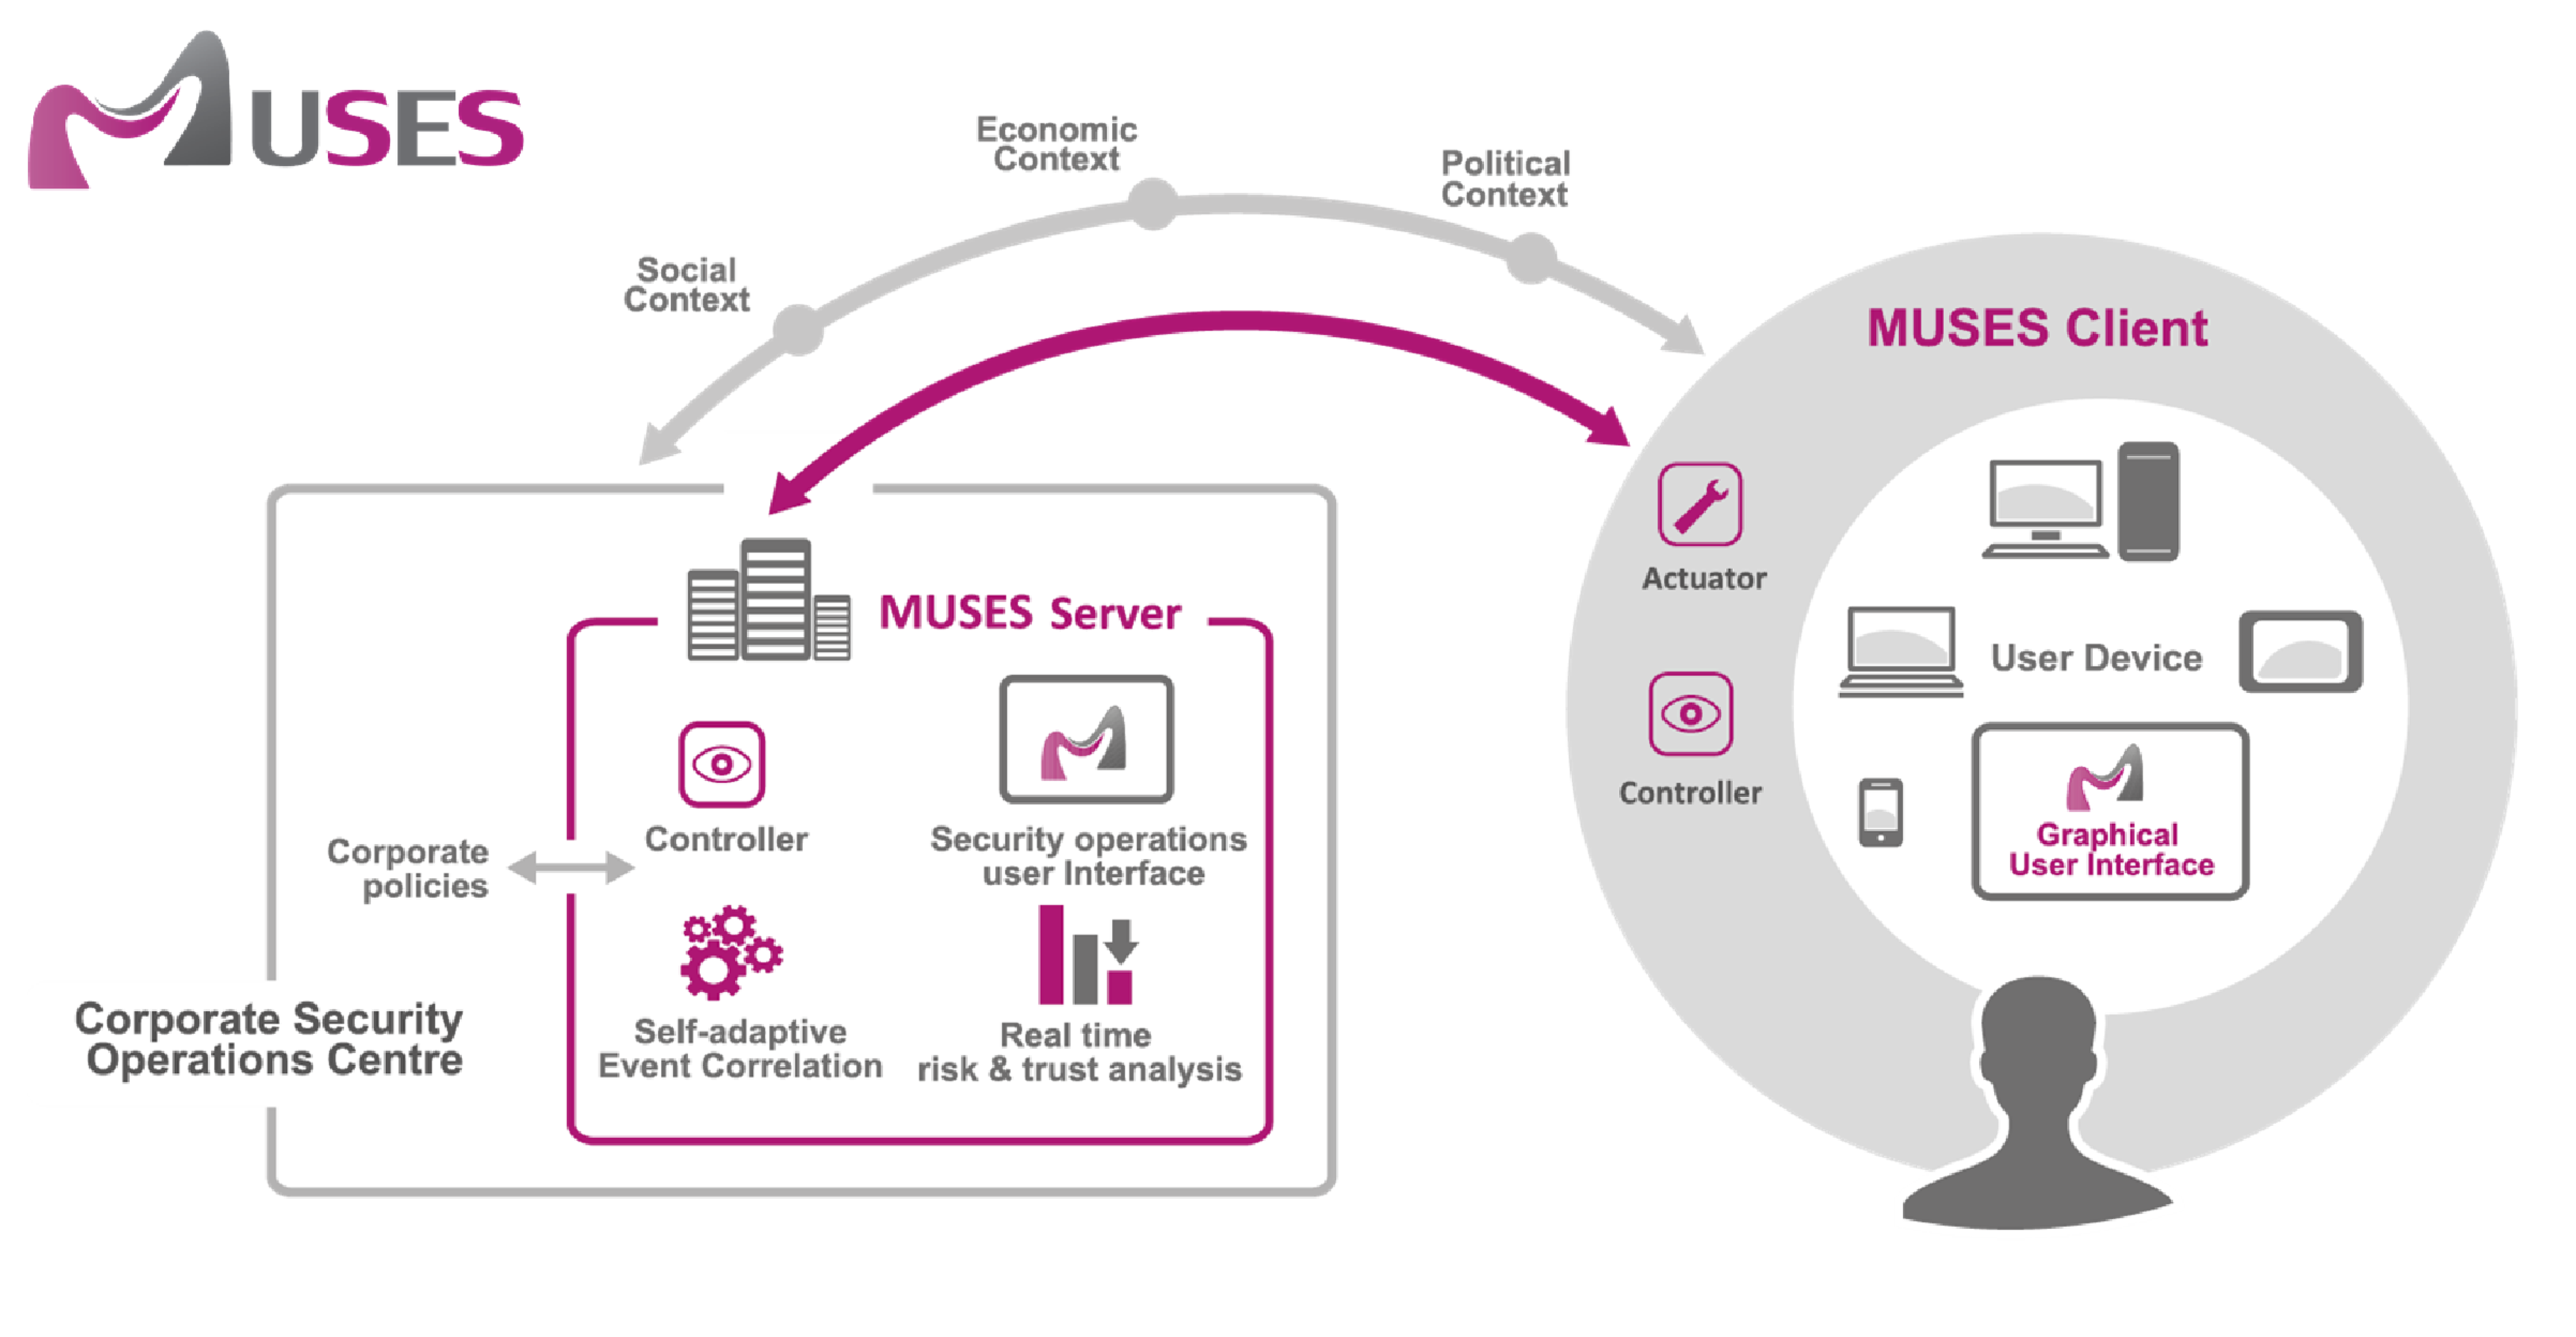
\includegraphics[scale=0.2]{img/system_overview.pdf}
\caption{MUSES system overview. Conceptual model designed by S2 Grupo.  http://www.s2grupo.es/.\label{fig:system_overview}}
\end{figure}

As a summary, this application includes two modules: a \textit{controller} and an \textit{actuator}. The former consists of a number of implemented \textit{sensors} in the device, which monitor the environment and the users' behavior \footnote{Which has been introduced as the `context' of an event.}. Then, the user's actions, as well as device configuration, or connection properties, are translated into a sequence of events. These events, along with the stored patterns defining the user's conduct, are processed by the system in real-time by means of a Risk and Trust Analysis Engine (RT2AE) and an Event Correlation module. Then, a decision is taken in the corporate Security Operations Centre (SOC) side, considering the RT2AE output and the set of security rules adapted to that specific user and context. The corresponding feedback is communicated to the user through the \textit{actuator}, and then the user decides to comply or not with the policy. As mentioned before, MUSES depends on the MUSES Aware applications to be able to really stop the application if the risk is dangerously high. In case that MUSES cannot kill the application process, and if the user decides to continue performing a risky action, the user trust value will decrease and the CSO will be notified.

MUSES architecture is shown in Figure \ref{fig:architecture}. % [Pedro] creo que la frase "suena mejor" sin "The designed" (pero es una apreciación subjetiva mía). % Agree
It is a \textit{client/server} approach in which the \textit{client} application can be installed in every user's mobile or portable device, independently of the platform. MUSES client is available up to date to be used in Android devices as well as in Windows mobile devices and PCs; the iOS client is under development. The same sensors are available in Android and Windows, but there is a strong limitation with monitoring iOS devices if they were not been \textit{jailbroken}. This means that if an iOS device has not been rooted, MUSES could not monitor every process in the device, and also it would have access only to some sensors. However, to be rooted is one of the situations that MUSES tries to avoid, which is why it depends on MUSES Aware apps. % [Pedro] ¿qué tal decir: "MUSES client is available up to date to be used in Android devices as well as in Windows mobile devices and PCs; the iOS client is under development."
% La verdad es que sí, la he releído y estaba muy mal redactada, qué vergüenza :(
As far as the server is concerned, it has been developed using Java to be installed with an Apache Tomcat in the corporate server, independently of its OS. % [Pedro] y respecto al servidor: "As far as the server is concerned, it has been developed using Java to be used with an Apache Tomcat in the corporate server." % Ok, cambiado y añadido lo del final.
Both sides are connected through a secure channel using HTTPS over the Internet. Figure \ref{fig:architecture} only shows the high-level components in each part, along with the way the information flows in the system. %FERGU: esto no se si es de muses y posiblemente esté por terminar, pero quitad las comillas raras

\begin{figure}[ht]
%\begin{center}
\hspace{-0.7in}
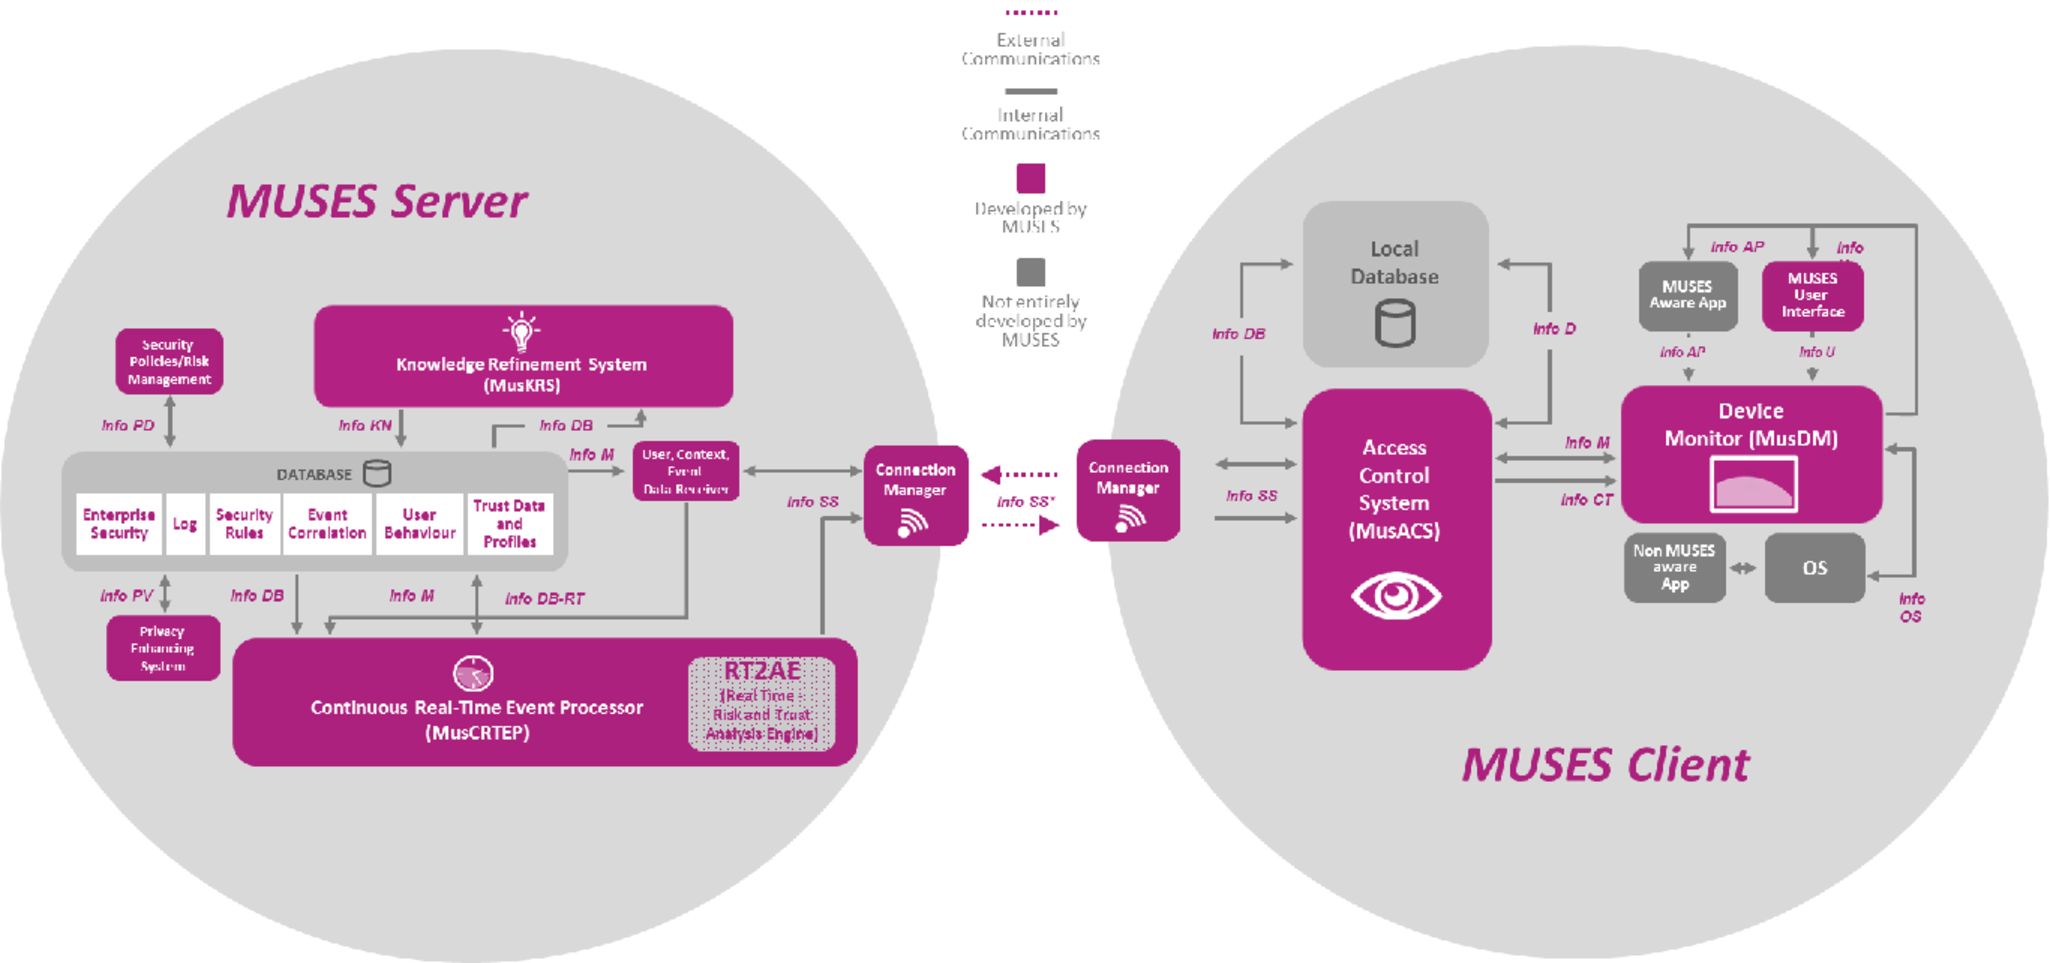
\includegraphics[scale=0.45]{img/architecture_modules.pdf}
%\includegraphics[scale=0.45]{img/muses_architecture.eps}
\caption{Design of the MUSES architecture (art by S2 Grupo). \label{fig:architecture}}
%\end{center}
\end{figure}

The use of a server is mainly based on the need of a powerful machine, able to work with massive amounts of data (\textit{Big Data}) \cite{BigData_11}, since the algorithms to apply to them require high computational costs \cite{Shirkhorshidi14Review}.
Moreover, part of the high computational cost methods to apply needs to be derived to this high-performance server, as the mobile devices do not count with enough computational power. These methods include DM \cite{DataMining_Lee01} and ML \cite{MachineLearning_Bishop06} techniques, which have been proved to be computationally expensive \cite{Cios07DataMining}. This server is also devoted to centralize the data gathering from all the devices in the company, composing a big database to which the commented techniques can be applied.

The system considers two working modes for every device: online and offline. In the \textit{online} mode the device can connect with the MUSES server, so that it can request the server to make a decision. On the other hand, in \textit{offline} mode the server cannot be reached by the device because there is not an available connection between them, so all the decisions are made locally.
This is done using an up-to-date copy on the Decision Table inside the Local database, which contains decisions for any type of detected event, along with the default actions to be performed if no rule is met. In this mode, the gathered information by the sensors in the device is stored for later submission to the server side when a connection is available, in order to be processed in the knowledge refinement process.
Moreover, when switching from offline to online mode, the device receives an updated copy of the Decision Rules, the so-called Device Policies, as a kind of antivirus database, in order to work again perfectly in offline mode if the connection is lost.

The MUSES system also performs an authentication process when the user logs in. The MUSES server authenticates to the MUSES client by means of a self-signed certificate. The authentication of the users is based on Spring Security, which is a Java EE framework that provides authentication, authorization and other security features for enterprise applications. When the user connects to the MUSES server for the first time, the MUSES client asks the server for the certificate, which is sent and installed in the client local database if the user credentials are right. As the user credentials are also stored in the MUSES client local database, the user can also log in to MUSES, and it therefore can apply the Device Policies. With regard to internal data security, MUSES makes use of the advantages that the OSs themselves offer to developers. More concretely, the first prototype for Android includes functionalities provided by the Android Application Sandbox \cite{blasing2010android}. This means that other applications cannot access MUSES data, nor even other developers. The only way to do this is by rooting the device, which is a state that MUSES can detect, and therefore warn about its implications. With regard to the encryption of the rest of the device data, MUSES stands for having a security policy which advices about the installation of existing open source tools \footnote{For instance, \url{https://github.com/neurodroid/cryptonite/blob/master/README.md}}, instead of having an own implementation.

% ----------------------------------------------------------

\subsection{Client/Device architecture}
\label{subsec:client}

There are three main components in this side:
\begin{itemize}
 	 \item \textit{Local Database}: it is a local security-based storage, which includes the set of security rules to be applied locally (Device Policies), user authentication data, and a cache of gathered events and information. The latter is useful when the device is in offline mode, so these events can be later submitted to the server side, when the device returns to online mode. 
%It contains the so-called \textit{Decision Table}, a set of rules in which the antecedents are high-level events, and the consequents are the corresponding decisions/actions, namely `allow', `deny' or `request' (the decision must be made in the server side).
 	 \item \textit{Device Monitor (MusDM)}: module which contains the two main described modules, controller and actuator. When a user performs an action, an event is automatically created and either sent to the server (online) or locally stored (offline). In addition, there are several sensors implemented in the system which periodically scan different aspects of the device configuration and the environment. This way, the system acts equally over specific actions, as well as when it detects something from the sensors that is against the security policies.
 	 \item \textit{Access Control System (MusACS)}: module in charge of making the decisions considering the gathered data. These decisions can be made locally if possible, or can be requested to the server if there is no rule which matches with the occurred events. 

%The subcomponents are the \textit{Decision Maker}, which performs the decision process; the \textit{User, Context, Event Handler}, which processes the events and information to be used for making the decision or stored for further submission (depending on the mode and on the gathered data); and the \textit{Security Policy Receiver} that updates the set of decisions (or Device Policies) in the Decision Table with those received from the server side, after an update or decision process.
\end{itemize}

The client is an important part of the a-priori risk treatment, because it both monitors the whole context, and finally acts or warns the user in event of a security violation. 
% Antonio - yo pienso que en este sistema cualquier violación de seguridad que se detecte se hará por medio de las reglas de seguridad. Eso sería lo ideal, pero para ello el CSO debe definir un conjunto que asegure la seguridad del sistema en la mayoría de casos. Luego el KRS podrá proponer nuevas reglas a través de 'predicciones' (inferencias) o refinamiento, pero estas últimas se construirán como reglas optimizadas para tratar con incidentes de seguridad ya detectados. No se pueden crear de la nada reglas para tratar con nuevos incidentes (desconocidos).
But security violations are mainly identified by security rules, which is why MUSES needs at least an initial set of rules, defined by the CSO. Then, it makes use of DM and CI techniques to improve or optimize them, enhancing the coverage. 
That is to say, the more sensors are implemented, the more information related to event context can be extracted. Implementing a sensor means to include a programmed method which triggers MUSES to start `listening' to some parts of a device. Then, the initial security rules establish which situations might cause a security violation, and the sensors provide with information which helps the MUSES server to identify events that are alike to the ones that are already known as dangerous.
% Antonio - esto no lo veo correcto. El meter más sensores no implica que se vayan a mejorar en mayor medida las reglas. Sino que se pueden controlar más formas de actuación de los usuarios.
% Yo o escribría como algo separado, por ejemplo "A way to enforce the security in these devices is the inclusion of more sensors, which would be able to detect more potentially dangerous behaviours by the users (and thus, security violations)" 
For these reasons, MUSES implements the following sensors:
% Para Pedro -> El caso es que "sensors" es su nombre dentro del sistema. ¿Estaría mejor su pusiésemos "monitoring sensors"?
% Antonio - yo quitaría el 'for this reason'

\begin{description}
  \item[Connectivity sensor:] It gathers all information related to network communications, in addition to security properties like network encryption, or number of neighbours. This allows MUSES actuator to forbid the user for sending important emails, or opening key assets if, for instance, the network encryption is not secure enough. 
  \item[Device protection sensor:] Which scans device security settings, such as the time until the device screen turns off, if the device has the screen protected with a password, or if the device is rooted \cite{hildenbrand2014}. This security mechanism adds the possibility of detecting security violations even if the user is not doing a specific action.
  \item[Location sensor:] User location can be obtained using the device GPS. Although, this might be taken against the preservation of user privacy. This is why MUSES allows the definition of a number of `zones', and therefore it only checks if the user is inside them or not, acting in consequence.
  \item[Mail sensor:] If the user is writing an email, MUSES client sensor can also check the email attributes. Thus, it can detect if the event context is dangerous, according to security policies and the RT2AE, before the mail is sent.
  % (Paloma) Pedro, aquí he cambiado el "is going to send" a "is writing" en vez de "is sending" porque en realidad lo que queremos es que se le avise antes de mandarlo, no cuando lo está mandando o lo ha mandado. Se explica después. ¿Cómo lo veis?
  \item[File sensor:] The type of file, also called \textit{asset}, is also very important for the application of security rules. Thus, this sensor aims to detect if some files might need more strict security policies, also depending on the rest of sensors.
  \item[App sensor:] It is in charge of monitoring the information about the application from which the user is performing the action, but also looks for installed trusted antivirus, and encryption applications. Additionally, this sensor gathers information about the applications which the user tries to install or uninstall.
\end{description}

It is important to note that MUSES does not work as an antivirus itself, but has a sensor which checks if the device has already an antivirus, and raises a security violation alert if not. It might happen then that the user ignores this advice and the device becomes compromised. As it would be explained in the next section, the sensors are constantly sending their monitored values, and therefore patterns are created, stored, and processed on the server. In case the device gets infected with rootkit-type malware \cite{bickford2010rootkits}, a sudden change in the values of the sensors will mean a significant change in the patterns. Then, this change in the patterns will be noticed by the server, which will immediately warn the user, and decrease the device trust value.

The rest of the components shown in the figure are: the \textit{MUSES User Interface (UI)}, the application through which the user interacts with the system; and the \textit{Connection Manager}, which controls the communications between MUSES client and MUSES server. 
In addition, there are two types of applications considered in this system. On the one hand, the \textit{MUSES Aware App} is an application adapted to MUSES, so the system can directly interact with it. This application must be implemented using the MUSES API (Application Program Interface). It should be noted that MUSES is an application that is running in the background, and third party apps can communicate with MUSES and ask for a response. Then, the MUSES API is not a normal API for building the third party application, but a collection of methods to allow this communication\footnote{The MUSES API is defined in the project, so for every application desired to be MUSES Aware, it should be implemented using this.}.
The main advantage of having MUSES Aware applications, is because actuator is able to actually forbid the users for doing something, if it implies a big risk for the company.

On the other hand, the \textit{Non MUSES Aware Apps} are those which MUSES cannot directly interact with. Usually, they can be accessed through the OS. But the type of information to gather from them and also the type of actions to do over them strongly vary depending on the OS, which should not be modified according to  \cite{Gessner13userfriendly}.
As was already mentioned, when MUSES is not able to close the application, a pop-up feedback message is automatically shown to the user. This message informs about why the action is considered as risky and what the user can do to avoid it.

% ----------------------------------------------------------

\subsection{Server architecture}

As in the client, we describe the three main components:
\begin{itemize}
	 \item \textit{System Database}: it stores all the information that the system can manage, including authentication data, enterprise security policies, values of the assets, 
% Antonio - no sé qué expresión será más correcta, pero deberíamos poner siempre "assets' values" o "values of the assets". Yo me inclino por la segunda.
user-related information (trust, context), events data, and, of course, security rules to apply with regard to the security policies.

	 \item \textit{Continuous Real-Time Event Processor (MusCRTEP)}: this component is the core of the MUSES system with respect to the decision making process. It includes an \textit{Event Processor}, the module in charge of performing the event correlation process \cite{deliverable21, deliverable52}. This is done by a so-called `Event correlation engine', which is in charge of taking the user action events that are sent from the device client, and analyzing them to look for an existing security rule that could be applied to the situation. The engine discovers that by analyzing the context events which are sent with the user action event, so that a complete model of the risks can be built. The output of this module is an `access request' which is sent to the \textit{RT2AE}. It considers the information included in the access request, as well as other information such as trust data and profiles, values of the assets, 
% Antonio - "values of the assets"
user reputation, or opportunity, to perform a risk and trust analysis task \cite{RT2AE_SOTICS13}. Finally, the RT2AE extracts the set of potential rules to consider in the analyzed situation, and these rules are therefore transformed into decisions (or Device Policies) and submitted to those devices to which they apply.

	 \item \textit{Knowledge Refinement System (MusKRS)}: this module is in charge of analyzing the information stored in the system database by means of Data Mining techniques, identifying relevant data, such as important patterns, key features, or security incidents. These are later processed for tuning up the existing set of rules, or for inferring new ones. The MusKRS component, along with the MusCRTEP, are what represent the extension of the state of the art in security solutions for a BYOD environment. 

\end{itemize}

There are some other components, which add extra functionalities to the system, namely:

\begin{itemize}
  \item A \textit{Security Policies/Risk Management} tool, that lets the company CSO to define and manage Security Policies and Rules in a friendly way. It also lets the management of risk-related information, useful for the RT2AE process, such as the values of the assets.
% Antonio - "values of the assets"
  \item  The \textit{Privacy Enhancing System}, which is a module aimed to fit with the legal compliance of the system regarding the user's data anonymization and retaining of these data in the system. There are three important points with relation to this matter \cite{deliverable72}. First, the data that the user provides to the system, such as name, or email, is only used for authentication purposes, so they are checked when the user logs in the system, but they are not used for Data Mining tasks. Then, the location of the device is never sent and stored in the database, but as stated in the previous section, there are a number of defined `zones'. What is checked is that the user is inside one of those zones of interest. For instance, a company might want to know if the user is inside or outside a zone defined as `company premises'. And finally, the use in MUSES of what is called as `soft limit' and `hard limit' \cite{deliverable72}. These limits exist to ensure the users that their data will not be kept longer than necessary. The soft limit is defined by the components that use the data (Event Processor, RT2AE, and Knowledge Refinement System) for decision making or rule refinement, but do not need that data anymore. In addition, the hard limit is provided by the law, in case that the employee leaves the company, or if there is a national law specifying a maximum data retention period.
  \item \textit{User, Context, Event Data Receiver}, which is devoted to receive data from the device side, such as events, or user-related data, and to distribute them among the components, storing in the database, and requesting the Event Processor to start the correlation task. Finally, there is another \textit{Connection Manager} which controls the communications with the device side. %FERGU: no usar etc en artículos, mejor poner: (events, user-related LOQUESEA, among others)
% Cambiado
\end{itemize}


% ----------------------------------------------------------

\subsection{Self-Adaptation in MUSES: The Knowledge Refinement System}

The self-adaptation, to the user and context, of the set of Corporate Security Rules is one of the main features of the MUSES system.
To this end, the \textit{MusKRS} module is in charge of analyzing all the gathered events, context, and user-related data. Then it processes the data and adapts or refines the security rules. This refinement is meant as an improvement of the existing security rules, and its aim is to deal with new, possibly insecure, events. As a result, a set of optimizations and additions to the set of security rules are proposed to the CSO of the company.

This procedure is composed by two main steps: first, a DM \cite{DataMining_Lee01} + ML \cite{MachineLearning_Bishop06} process is performed in the \textit{Data Miner} sub-component; second, a refinement and inference process is done in the \textit{Knowledge Compiler} sub-component, using the data that was extracted in the first step, and by means of CI techniques.
The refinement or adaptation of the security rules can be made through techniques as simpler as generalization or specialization of rules, for instance, or by more complex CI methods such as Evolutionary Algorithms \cite{EAs_Back96}.

Another important fact is that MUSES functionalities are completed by a human controller, normally the CSO, who supervises the system activity by means of a graphic interface they can interact with. 
% Antonio - Si estamos hablando en tercera persona del singular se suele poner 'she' para referirnos a una persona de cualquier sexo, pero me gusta más poner 'he/she' para no discriminar. En todo caso intentaré poner 'they' en lugar de 'he/she', pero aquí, tal y como está redactado 'they' no queda bien por el verbo. 
% Antonio - No lo cambio porque no sé tu opinión, no es por dar trabajo extra.
% A ver, este fenómeno gramático se llama "singular they", y se considera más correcto utilizarlo que poner "he/she". No es que me lo haya inventado yo :\
% Antonio - Ok, entendido. Es que nunca lo habia visto.
Thus, adapted and inferred security rules are not directly added to the current set of rules, but they are proposed instead as draft rules to this human controller, in order to be accepted if they are interesting and useful. The system also uses the acceptance or rejection of new rules as `feedback`, learning from these decisions, and refining the rules according to this.

The following sections describe these processes: first, focusing on DM techniques to be used both automatically by the MusKRS, and by the mentioned graphic interface for showing useful information to the CSO; second, used CI techniques are explained, mainly focusing in Evolutionary Computation (EC) \cite{EAs_Back96} approaches. EC methods have demonstrated to have a good performance, and have been widely used in security-based environments for solving security issues, such as intrusion detection \cite{GA_intrusion-majeed}, design and evaluation of security protocols \cite{GP_intrusion-lu,GA_networksecurity-zarza}, or for the optimization of different aspects related with security: IT security costs \cite{EAs_securitycosts-kirta}, and cryptographic protocols \cite{GA_cryptographicprotocols-zarza2}, among others.

% ------------------------------------------------------------------
%
\subsubsection{Data Mining + Machine Learning}
\label{subsubsec:dm_ml}

This task is performed by the \textit{Data Miner} module. It  takes the `raw' data from the database and processes the information, in order to yield a set of relevant data for the Knowledge Compiler module and for the human controller. In the first case, this Data Miner component takes the set of data as a reference for refining or adapting the current set of security rules, to deal with anomalous situations, for instance.

The set of data is composed by the so-called patterns, which consist of an occurred event 
% Antonio - quedaba raro decir que estaba formado por 'un evento' como tal
and all the related information to that event. This means that the context in which the event was, is translated into a number of \textit{attributes} of the pattern. 
%This process is mainly non-supervised. 
% Antonio - Lo que es no supervisado es la clasificación, pero si se está explicando de otra forma ya no tiene sentido decirlo.
Moreover, a lot of attributes are extracted from the events, for obtaining the more information as possible. 
During the first trials, a mean of 201 events per day and user was observed. By considering just a medium size company, of 250 employees, that would make an average of 50300 events per day, of which a high number of features are extracted. Furthermore, if for instance 6 months are considered for the `hard limit' (see previous section), the amount of events to be processed would exponentially grow, until reaching the 9 million events. For even bigger companies, this all result in huge datasets, so that MUSES makes use of several Big Data processing methods \cite{BigData_11}, such as: 

\begin{itemize}

\item \textit{Pattern Mining} \cite{PatternMining_Han07}: 
From the whole set of patterns which form the built dataset, the most frequent, as well as the uncommon, are obtained. The idea is that infrequent patterns are potentially suspicious, and thus, could be of interest to be checked by the CSO, or to serve as a reference for the rule-refinement process.

\item \textit{Classification} \cite{classification_67}: 
This technique tries to train a model (classifier) able to associate every pattern in the dataset to a class, so that the model could be used for assigning a class for further incoming patterns with an unknown category.
Then, the model learns from events that, according to the ISPs, had been previously marked as `allowed' or `denied'. When a new event arrives to the server, if it has not an assigned decision, the classifier should provide one based on the similarity with previous, and already labeled, patterns.

\item \textit{Clustering} \cite{Clustering_Jain99}: 
The aim of this method is grouping the patterns considering some similarity criteria, in order to manage them as a set. This is used for providing data visualization mechanisms through a graphical interface. This would make easier to interpret data interaction and the distribution in clusters with respect to the different attributes, or features, of the patterns.

\item \textit{Feature Selection} \cite{FeatureSelection_Guyon03}: 
It consists of extracting the most important variables from the data. Feature selection techniques have been proven \cite{liu1998feature} to preserve the performance of the original feature set 
% Antonio - yo pondría 'quality' en lugar de 'performance'. Un dataset no tiene rendimiento, bajo mi punto de vista
in terms of classification accuracies, while significantly improve the processing time.

\item \textit{Data Analysis}: 
This provides the CSO with mechanisms to visualize interesting facts about the data, such as most frequent events, dangerous or suspicious users according to their behavior, most triggered rules, etc. All this information is shown to the CSO via the mentioned graphical interface, implemented in the server.

\end{itemize}

%\pagebreak

% ------------------------------------------------------------------
%
\subsubsection{Computational Intelligence: Evolutionary Computation Methods}
\label{subsec:ci}


MUSES uses different EC approaches, initially, two in the DM/ML part of the process, and three in the rule-refinement and adaptation phase. They are based on Genetic Programming (GP) \cite{GP_Koza92}, and Genetic Algorithms (GAs) \cite{GAs_Goldberg89}.

The Data Miner module adopts two evolutionary-based approaches. In the first place, a \textit{GP-based classification} method. This is useful for two main reasons: to deal with the data class imbalance \cite{imbalance_techniques_02}, which is very common in classification problems with real systems, gathering real data; and to better manage categorical data, since most of the features and information gathered from the events take these kind of values.
%, and being non-numeric does not allow to measure the distance between them.
% Antonio - claro que se puede medir la distancia entre valores no numéricos, lo que pasa es que normalmente, ésta no es representativa. Mejor omitir esto o poner de forma genérica que 'los valores categóricos dificultan el proceso de machine learning'.

Thus, this kind of classification method is able to manage unbalanced datasets, for instance, by considering a fitness function in which a cost is associated with the classifier accuracy at every iteration, having a penalty cost when the classifier makes a false negative. A false negative is an element from the minority class which is classified as belonging to the majority class \cite{cost_adjustment_07}.
With regard to the type of data, since GP algorithms can manage rule or tree based models, it works perfectly with any categorical feature, yielding a good classifier as it has been demonstrated in \cite{cost_adjustment_07}.

The second evolutionary approach taken in the Data Miner is the Feature Selection process that was mentioned in the previous section. This process is conducted using a GA as a meta-algorithm to test all the possible combinations of pattern features in the classification. Thus, the GA algorithm can optimize the group of features to be considered in the classification task, improving both the computational time of this task and also the obtained accuracy of the method \cite{liu1998feature}.

On the other hand, the refinement or adaptation of the security rules is performed by the \textit{Knowledge Compiler} module, and it uses three EC methods. These methods can be used for inference and optimization, and they use different data as part of the process, such as:
% [Pedro] maybe we should specify how the following data is used in each one of the 3 EC methods...

\begin{itemize}

\item The information extracted from the Data Miner sub-component, mainly concerning the anomalous, unclassified or misclassified patterns. These are those patterns which did not match with any of the existing classes, as they are quite different from the patterns belonging to those classes. This way, they cannot be included in any of the classes and thus they should be taken into account for a potential inference or update in the set of security rules, in order to `cover' them.

\item User-related information, and context information in general, corresponding to those anomalous or unlabeled events. Thus, the user's location zone, role, or device settings, for instance, can be considered in order to select the applicable set of rules for those conditions.

\item Risk information extracted from the user profile, e.g. ``Did the user received a lot of `denies' or `allows' before?'', in other words, ``Is the user trustworthy?''. In case the user is not, meaning that the user trust value is low, more restrictive rules can be created, otherwise the corresponding rules could be `softer' for that user.

\item The information about the user behavior with respect to system messages, whether the users acts in consequence or against MUSES advice, as well as user feedback. The user feedback has been measured in the MUSES trials by making interviews with the people who have used MUSES, but it can also be measured by pop-up messages, such as ``has this information been useful?''. 
% Antonio - quito el guión porque un revisor dice que se usan demasiados y que hacen el texto menos fluído y legible.
% Paloma -  "forward slash" no significa guión. Un forward slash es un / que sí había muchos en el texto.
% Antonio- Ok. En todo caso lo dejaría sin el '-type', pero como veas. Si lo quieres poner como estaba, el ', such as' lo añadí yo y lo mismo no queda bien así. 
% Ok pues con el such as.
All this information contributes to the inference of new rules or in adaptation, in order to deal with, for instance, users that repeatedly ignored warning messages.
Moreover, important log information with regard to the parameters used or the decisions made in the different modules can be used for further tests of new inferred rules, as it is explained below.

\end{itemize}

As the rule refinement process is considered of the same importance as inferring new ones, the following three approaches have been implemented:
% [Pedro] I'd change this to: "As the rule refinement process is considered of the same importance as inferring new ones, the following three approaches have been implemented:"
% or even to:
% "Due to the importance of the refinement process (it is considered of the same importance as inferring new ones) the following three approaches have been implemented:"

\begin{itemize}

\item A \textit{GP rule inference} method, which generates new rules in order to `cover' those situations that have been not contemplated in the current set of rules. Thus, a new rule would be created for dealing with the patterns to which the classifier could not assign a class.
The generation of new rules is done by considering the so-called \textit{dictionary}, i.e. a set of terms corresponding to all the possible context situations and user actions in the system, which are the antecedents and consequents \footnote{The antecedents are the conditions of a rule that have to be met to apply the consequents.} of the security rules to be inferred.
The evaluation of these rules is done by considering the information that has been described. Thus, it is possible to `simulate' the whole system behavior when the new rule is included. Therefore, the system gets a value of its performance in terms of, for instance, how many of the events that were not classified or misclassified, are covered now. As was also mentioned, the user or device trust values influence the creation of the rules.
Finally, the inferred rules are proposed to the CSO as ``new, but not yet refined'', along with their evaluated performance.

\item A \textit{GP rule refinement} approach, which optimizes the current set of rules, adjusting the values in the conditions. The set of rules that could be refined is composed by the new rules from the GP-based inference, but also by the original set of rules which was already completed by the Data Miner. Thus, some superfluous parts of the rules and even complete rules could be removed or improved, obtaining for instance specializations or generalizations of existing rules which could lead to a better performance. % [Pedro] change "could mean a better" to "could lead to a better"
The evaluation of the whole set of security rules is done by considering the number of unlabelled patterns that are `covered' after the adjustments. Again, the rules at the end of this step are presented to the CSO as ``refined''. The CSO is the one who decides, according to the performance simulation results, if an inferred rule, or the refined one, is the rule which is finally included in the system.

\item A \textit{GA optimization} algorithm for adapting the values of the assets. %FERGU: "values of the assets" mejor? Los valores no son "poseidos" por los assets, no? xD (tampoco tengo mucha idea del genitivo sajón, ojo)
% Toda la razón :D Se ma colao, shame on me!
These are numerical representations of the importance of the corporate assets, and are considered in the Real-Time Risk and Trust Analysis process, in order to assign a risk value to every potential decision that can be made by the system.
By evaluating the partial solutions proposed by the GA, this approach provides the CSO, who is in charge of assigning and adjusting these values over time, with information about the most dangerous situations for certain assets. In this process, then, the context information that is gathered by the system is very important. %FERGU: pondría el "in this process" al principio de la frase. % Ok, cambiado
The adaptation or adjustment concerns the change in the value that an asset has due to a loss of importance, for instance, for being an out-to-date document.

\end{itemize}

% [Pedro] it is not clear for me whether those 3 methods can be used (are used) independiently or one after the other(s).

As a summary, the Knowledge Compiler module uses two EC-based processes for inferring and refining rules, plus another one for adjusting values of the assets.
% Antonio - "values of the assets"
 Both the inferred rules and the refined rules are presented to the CSO, who includes them or not in the system, and this acceptance or rejection acts itself as a feedback for future rule inference.


% ---------------------------------------------------

% Antonio - pongo esto en una sección nueva para que destaque más. Es muy importante para los revisores. Por favor Paloma, revisa si lo que he puesto es correcto (número de usuarios y demás).
\subsection{Trials and tests of MUSES}
\label{subsec:trials}

A MUSES first prototype, implemented for Android devices, has been recently tested. These trials have been conducted in an actual Spanish company, with 50 employees using the system on their own devices.
% He quitado "(a partner in the European Project where the system is being developed)" porque creo que es irrelevante, y si no se puede redactar de manera que esté fuera de los paréntesis, no debería estar.
The trials were divided in two phases: \textit{silent} and \textit{verbose}, 1 month duration each. During the \textit{silent} phase, MUSES was able to gather data, but without warning the users when a security incident was happening. A total of 23358 security violations were detected. In the \textit{verbose} stage, MUSES started to show warning pop-ups to the users, every time a security incident happened. 

As results, not only the number of security violations were reduced by half in the first two weeks (10977), but the number went on decreasing until it was 0 even before the trials period finished. Thus, we can assume that MUSES is an effective tool, even though it has the limitation of needing an initial set of defined security rules to start working (this will be better explained in Section \ref{sec:comparison}). For this, MUSES also includes a set of guidelines for the companies to build adequate security policies. For instance, the set of initially defined rules used for the trials included a blacklist of forbidden applications, a whitelist of allowed ones, and requirement of antivirus, among others.

With respect to the computational costs, in this first prototype it takes less than 0.5 seconds in the client side, if there is already a decision in the local table for the happened event. Otherwise, i.e. if there is need to ask the server to make a decision (by means of Event Correlation + Risk and Trust Analysis), the time grows up to 2.5 seconds in the worst case.

\section{MUSES Advantages over Other Solutions. Beyond the State of the Art}
\label{sec:comparison}

MUSES is mainly a free, open-source, platform independent solution, and adopts the recommended best practices by Romer \cite{Romer14BestPractices}. %Está bien aquí Fergu?
These features make it a good alternative to most of the proprietary, close and system-specific tools presented in Section \ref{sec:toolsreview} (all but WSO2). In addition, most of the existing tools take into account only smartphones and tablets, but MUSES also covers laptops and company PCs, thus, it is not only for BYOD. Moreover, the companies which might want to work with one of the reviewed systems need a specific operating system in the server, being even more restrictive in some cases. This is specially remarkable in the case of the Blackphone, forcing the companies and the employees to purchase a specific device. MUSES is a good solution towards these cases, since it is a multi-platform system in both the client and the server. 
Table \ref{tab:taxonomy} summarizes the features of the main analyzed tools, with respect to the proposed taxonomy in Section \ref{sec:toolsreview}. Also, Table \ref{tab:features} shows the features of the analyzed products considering licenses, type of supported devices, and price.
% Antonio - Antares, ¿podrías incluir en la comparativa las otras herramientas que se han analizado? Las de Citrix, WSO2, Azzurri, Good...

\begin{table}[ht]
\begin{footnotesize}
  \centering
  \renewcommand{\arraystretch}{2.0}% Spread rows out...
%  \resizebox{12cm}{!}{
  \begin{tabular}{>{\centering\bfseries}m{0.6in} >{\centering}m{0.6in} >{\centering}m{0.6in} >{\centering}m{0.6in} >{\centering}m{0.6in} >{\centering\arraybackslash}m{0.6in}}
    \toprule
      & \textbf{Offline threat detection method} & \textbf{Updatable database} & \textbf{Standalone} & \textbf{Non-invasive data access} & \textbf{Superuser system control} \\
    \midrule
    MUSES & \cmark & \cmark & \cmark & \cmark & \cmark  \\
     \arrayrulecolor[gray]{0.6}\hline
    IBM Mobile Security & \xmark & \xmark & \cmark & \xmark & \xmark  \\
     \arrayrulecolor[gray]{0.6}\hline
    Sophos Mobile Control & \cmark & \xmark & \cmark & \xmark & \xmark \\
     \arrayrulecolor[gray]{0.6}\hline
    Samsung Knox & \cmark & \xmark & \cmark & \cmark & \cmark\\
     \arrayrulecolor[gray]{0.6}\hline
     Blackbery Balance & \xmark & \xmark & \cmark & \cmark & \cmark\\
     \arrayrulecolor[gray]{0.6}\hline
    Blackphone & \nmark & \nmark & \cmark & \cmark & \cmark\\
     \arrayrulecolor[gray]{0.6}\hline
    Android for Work & \cmark & \xmark & \cmark & \cmark & \cmark\\
    \bottomrule
  \end{tabular}
%  }
\end{footnotesize}
  \caption{Features of the analyzed tools with regard to the proposed taxonomy to classify BYOD systems (see Section \ref{sec:toolsreview}).}
  \label{tab:taxonomy}
\end{table}

\begin{table}[ht]
\begin{footnotesize}
  \centering
  \renewcommand{\arraystretch}{1.8}% Spread rows out...
%  \resizebox{8cm}{!}{
  \begin{tabular}{>{\centering\bfseries}m{1in} >{\centering}m{1in} >{\centering}m{1in} >{\centering\arraybackslash}m{1in}}
       \toprule
      & \textbf{License} & \textbf{Devices} & \textbf{Price} \\
       \midrule
    MUSES & OpenSource & Android, Windows 8.1, Windows Phone, iOS & Free  \\
       \arrayrulecolor[gray]{0.8}\hline
    IBM Mobile Security & Proprietary & iOS, Android, Windows Phone, Blackberry  &  By Request\\\\
        \arrayrulecolor[gray]{0.8}\hline
    Sophos Mobile Control & Proprietary & iOS, Android, Windows Phone  &  By Request\\
        \arrayrulecolor[gray]{0.8}\hline
    Samsung Knox and Blackbery Balance & Proprietary & Android Samsung Devices and iOS & 12\$ per year/device \\
        \arrayrulecolor[gray]{0.8}\hline
    Blackphone & Proprietary & Own device & 120\$ per year \\
        \arrayrulecolor[gray]{0.8}\hline
    Android for Work & Proprietary & Android and devices with Chrome Browser &  12\$ per month/user\\
       \bottomrule
  \end{tabular}
%  }
\end{footnotesize}
  \caption{Features of the analyzed products considering licenses, type of devices and OS, and price.}
  \label{tab:features}
\end{table}
% Antonio - Antares, ¿no había más tablas?
% Por favor, que alguien rellene los datos de la solución de IBM. ¿Fergu?¿Antares?
% Quizá habría que indicar que MUSES se puede instalar en PC también en la tabla. ¿Sabéis si los demás se puede o son sólo para smartphones/tablets?


Another comparison would be that the existing products are mostly policy-based, while MUSES makes its decisions not only considering policies, but also based on the terminals and users context, such as connection properties, or trust value of the device, to really understand the real risk that comes with a specific action.

Also related to this issue, a very big advantage of the MUSES system that is not present in the other solutions is its self-adaptivity power. The proposed system uses different methods to create new security rules, being their aim to cover new vulnerabilities or threats. Thus, MUSES is able to adapt to changes by applying classification techniques to create new rules, and then refining the whole set of existing policies. Additionally, MUSES is able to discover new threats by a combination of real-time risk and trust analysis plus a classifier trained with all the occurred events in the system.

However, MUSES presents a limitation regarding the enhance of rules,
since, in principle, it cannot predict or generate rules for dealing
with unexpected or unknown events, which could lead to a security
incident. The philosophy is that the initial set of rules, defined by
the CSO, should be very restrictive regarding possible unexpected
users' behaviours or events, in order to avoid as much security
incidents as possible. As the system works, MUSES would be able to
define new rules through refinement which could get an associated
decision after the corresponding events have happened. Thus, this will
lead to obtaining an optimal set of security rules.

In addition, MUSES can also infer or create new rules using computational intelligence techniques. These rules could deal with unexpected situations not previously happened, but must be previously approved by the CSO. Of course, everything is constrained by the available set of sensors which, in turn, define the possible information that MUSES will analyze and use in the refinement and inference processes.

Moreover, another clear improvement over the rest is that MUSES can work in both online and offline modes, depending on the client being able to connect with the server or not, which favours the real-time decision making process.

These are not only advantages of MUSES over the existing products, but also a progress beyond the state of the art in some fields like risk and trust analysis, event correlation, and human-computer interaction (HCI).

First, as mentioned previously, it  implements a self-adaptive event correlation, including a novel hybrid technique of rule refinement and rule adjustment extracting relevant information from processing huge amounts of data. Then, the project defines a new approach to risk management taking into account threats, with their costs, as well as the innovative concept of opportunity \footnote{The following beneficial outcome from a situation on which, for instance, a user is able to work while waiting at the airport if the risk is low enough.}. 

As far as the HCI is concerned, in Section \ref{sec:preliminaryconcepts} we talked about how it has been demonstrated by Shaw et al. \cite{SecPolComp09} and Herath et al. \cite{SecPolPenalty09} that the compliance of the employees of a company, with respect to the security policies, increases by educating them and decreases by punishing them. Therefore, the fact that MUSES is focused in avoiding security incidents due to users' unawareness of the ISPs, it sets up a significant advance in the state of the art. This is because not only the incident is avoided, but the user is educated, which at the same time avoids future risky situations.
With regard to device monitoring, MUSES  also take into account the so-called context observation, by which private or professional scenarios can be detected, or predicted, based on advanced machine learning techniques. Finally, the project is concerned about legal compliance in regards of Information Security Policies, so that it  contributes to the proposal for the EU Data Protection: legal binding force and legal certainty of company policies, and end-user responsibility.

With regard to the scientific contribution of the system, one of the main differences with respect to previous works is the consideration of security threats `brought' by the user's behavior inside the system, i.e. through interaction or events, rather than more general and external threats. Moreover, the techniques to be used in MUSES  works with real data, as a difference to several research works which consider simulated data.

Authors have used DM techniques in previous works, but usually aiming for a specific general objective, for instance the detection of threats such as botnet \cite{botnet_detection_clustering_09}, or the recognition of anomalies \cite{feature_selection_anomalies_08}. However, these works do not contemplate any process to improve the system as the refinement phase in MUSES.

There are some proposals in which security policies are inferred or refined \cite{inferring_policies_socialnetworks_09,policy_generation_clustering_10}, but they do not affect the ISPs as in MUSES, and they are not based on the user's behaviour in order to do this.

GP has been previously proposed in bibliography \cite{rule_generation_gp_09,sec_policy_evolution_gp_08}, even for creating new policies or rules in a security-aimed sense. In any case they do not affect the ISPs and moreover, our proposed evaluation functions, completely integrated in the system, for the refinement and inference approaches are novel.

With respect to GA, they have been extensively used in this scope in the literature, mainly for the detection of anomalies and intrusions rather than for optimization, as it is used in the proposed system. However, there are some examples that could be used as model for our approach, such as \cite{EAs_securitycosts-kirta,risk_reduction_ga_12}.
